\section{Toy experiments of $CL_s$ and $CL_{s+b}$}
\label{S. CLs In Action}

We have introduced the $CL_{s+b}$ and $CL_s$ methods and discussed their important properties. Now we implement a simple test-case from which to demonstrate them in practice.


\subsection{Defining the models}
\label{S. CLsInAction::Models}

Say that we measure event yields in bins $i$ of some nameless observable. We have miraculously been able to perform these measurements with no systematic uncertainties. However, they are nonetheless subject to statistical fluctuations around the expected event yields. We have one source of background, which follows a continuous distribution as a function of our observable. We are searching for a bump in this spectrum which we want to interpret as a signal of a dark matter mediator. We claim that we know the background and signal distributions exactly (no systematic uncertainties!), but we do not know anything about their respective rates. The expected event yield in bin $i$ is
\begin{equation}
\nu^\text{exp}_{\text{evt, }i}\left(\mu_\text{sig}, \mu_\text{bkg}\right) = \mu_\text{sig} \cdot \mathcal{S}\left(i\right) + \mu_\text{bkg} \cdot \mathcal{B}\left(i\right)
\label{E. ModelYields}
\end{equation}
where $\mathcal{S}$ is a signal template (known), $\mu_\text{sig}$ is a signal scale factor (unknown),  $\mathcal{B}$ is a background template (known) and $\mu_\text{bkg}$ is its scale factor (unknown). Figure~\ref{F. Asimovs} shows two possible models. Black points are an Asimov dataset, meaning that each measurement has been set to its expected value with an uncertainty reflecting its expected variance. We are performing a counting experiment, so we estimate uncertainties to have a magnitude of $\sqrt{\nu^\text{exp}_{\text{evt, }i}}$ (because we expect them to be Poisson distributed). \texttt{Model 1} has a moderate background rate which allows a non-negligible sensitivity to the signals when $\mu_\text{sig}^\text{true}=1$. \texttt{Model 2} has exactly the same signal and background templates but a signficantly larger background rate.

%This will be used to demonstrate the behaviour used to motivate use of the $CL_s$ method in the previous section.

\begin{figure}[t!]
\centering
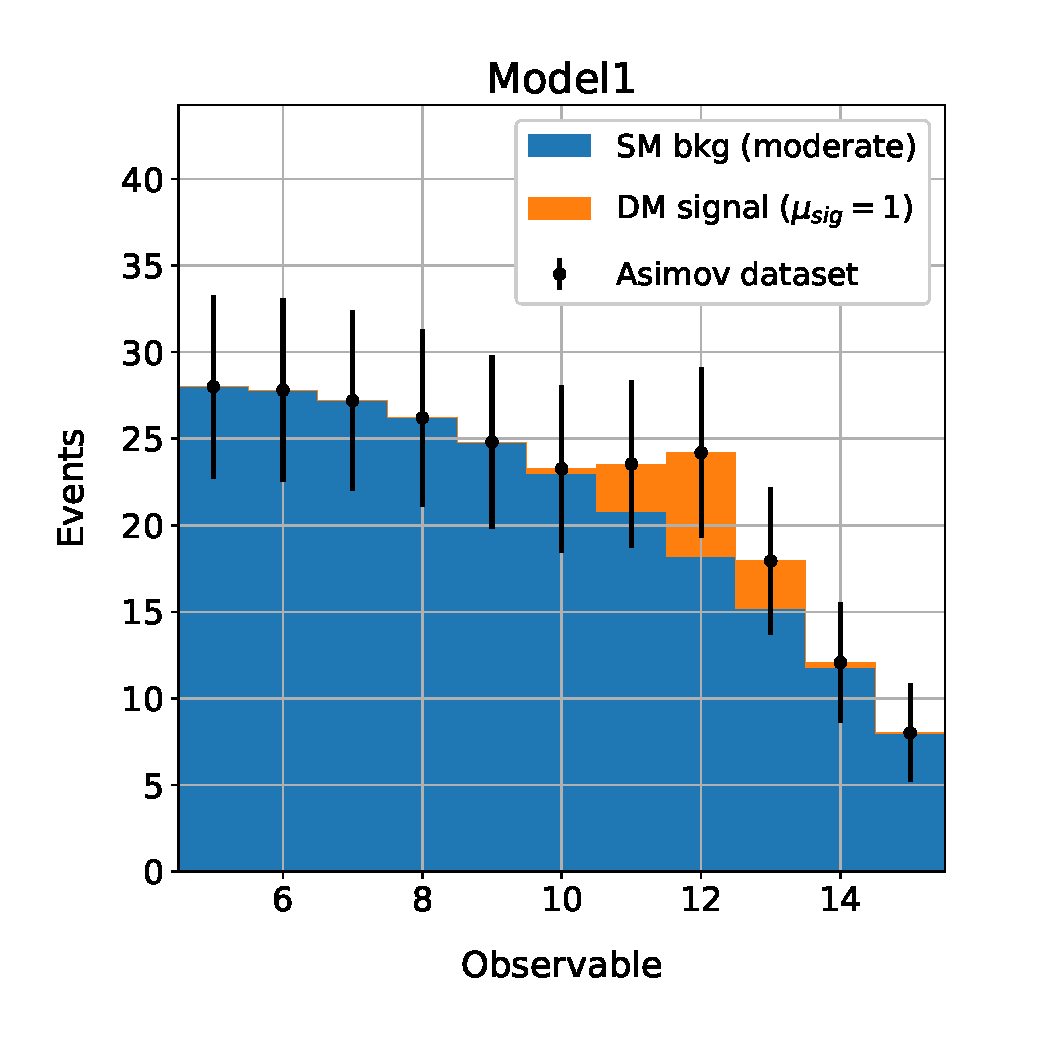
\includegraphics[page=1, width=0.49\textwidth]{ModelDatasets.pdf}
\includegraphics[page=2, width=0.49\textwidth]{ModelDatasets.pdf}
\caption{Left: Asimov dataset for an experiment with $\mu_\text{sig}^\text{true}=1,~\mu_\text{bkg}^\text{true}=0.8$. Right: Asimov dataset for an experiment with $\mu_\text{sig}^\text{true}=1,~\mu_\text{bkg}^\text{true}=5$.}
\label{F. Asimovs}
\end{figure}





\subsection{Defining the likelihood}
\label{S. CLsInAction::Likelihood}

We now define likelihood functions for the $s+b$ and $b$ models. This is easy for event counting experiments without systematic uncertainties. The templates $\mathcal{S}$ and $\mathcal{B}$ are known exactly\footnote{We stress that this is only a result of us not considering systematic uncertainties. In general any lack of model knowledge will be accounted for using NPs.}, perhaps derived in practice using Monte Carlo simulations, but defined here using some arbitrary functions we invented. The expected probability for observing $\nu^\text{obs}_{\text{evt, }i}$ events in bin $i$ follows a Poisson distribution around the expected mean in that bin, $\nu^\text{exp}_{\text{evt, }i}$. Since our bins are statistically independent, the \textit{combined probability} is simply the product of the individual bins. Therefore
\begin{equation}
\begin{aligned}
\mathcal{L}_{s+b} \left(\mu_\text{sig}, \mu_\text{bkg}\right) &=   \text{Poisson}\left( ~ \nu^\text{obs}_{\text{evt, }i}  ~|~  \nu^\text{exp}_{\text{evt, }i} \left(\mu_\text{sig}, \mu_\text{bkg} \right) ~ \right) \\
\mathcal{L}_{b} \left(\mu_\text{bkg}\right) &=   \text{Poisson}\left( ~ \nu^\text{obs}_{\text{evt, }i}  ~|~  \nu^\text{exp}_{\text{evt, }i} \left(0, \mu_\text{bkg} \right) ~ \right) \\
\end{aligned}
\end{equation}
where $\nu^\text{exp}_{\text{evt, }i}$ is defined according to Eq.~\ref{E. ModelYields}. We note an interesting property. In the \textit{asymptotic limit}, which is the limit of infinite event yields (achieved by an experiment with infinite integrated luminosity and $\nu^\text{exp}_{\text{evt, }i}>0 ~\forall~ i$), a Poisson distribution tends towards a Gaussian one. For large datasets, the quantity $-2 \ln \mathcal{L}$ is then expected to follow a $\chi^2$ distribution with degrees of freedom equal to the number of measurements ($N_\text{bins}$). The optimisation process for $-2 \ln \mathcal{L}^\text{max}$ will remove some degrees of freedom. Now, if the $s+b$ and $b$ models are identical but for the inclusion of several \textit{PoIs} in the $s+b$ model, as is true for our model, we find a nice result: $-2 \ln q$ in the asymptotic limit represents a $\Delta \chi^2$ distribution with the number of degrees of freedom equal to the number of PoIs.

For the experiment shown in Figure~\ref{F. Asimovs}, we do not always measure enough events to rely on the asymptotic approximation, and so we will not assume $-2 \ln q$ to be a $\Delta \chi^2$ distribution. However, this fact is too useful not to be mentioned: it will come up very often, and can be used to construct a test statistic $q\sim\exp\left(-\frac{1}{2} \chi^2\right)$ from a set of normally-distributed measurements with known covariance.






\subsection{Bias and coverage of the fit}
\label{S. CLsInAction::BiasCoverage}

An experiment is unbiased if the mean $\langle \vec{\hat{m}} \rangle$ of many repeated estimates $\vec{\hat{m}}$ of some quantity $m$ is equal to its true value $m_\text{true}$. For an unbiased method, Gaussian uncertainty estimates of magnitude $\vec{\hat{\sigma}}$ have the correct coverage if $m_\text{true}$ is contained within the interval bounded by $\hat m_k \pm N\hat\sigma_k$ with the frequency expected by integrating a standard normal distribution over the interval $[-N,N]$, where $k$ labels individual estimates.

We now introduce the concept of a \textbf{pull}. Say that we perform a large number of experiments and calculate
\begin{equation}
\hat p_k = \frac{\hat \mu_k - \mu_\text{ref}}{\hat \sigma_k}
\end{equation}
for each one. We expect that $\hat p$ will be normally distributed around $\left(\mu_\text{true}-\mu_\text{ref}\right)$ provided that our measurement is unbiased and has well estimated Gaussian uncertainties.

We can use this fact to test the bias and coverage of our method. We want to generate an ensemble of estimates and check that the resulting $\vec{\hat{p}}$ have the expected mean and variance. This does not require us to perform our experiment multiple times. Instead we use \textbf{toy datasets} (a.k.a. psuedo-experiments) using the following process.

\begin{figure}[t!]
\centering
\includegraphics[page=3, width=0.49\textwidth]{ModelDatasets.pdf}
\includegraphics[page=4, width=0.49\textwidth]{ModelDatasets.pdf}
\caption{Toy datasets generated for the (left) model 1 and (right) model 2 experiments. Each toy represents a possible statistical fluctuation around the expectation. Toys are generate following the expected Poisson probability distributions. A collection of toys therefore represents a representative sampling of the ensemble of all possible datasets.}
\label{F. Toys}
\end{figure}

In Figure~\ref{F. Asimovs}, we presented an Asimov dataset around the expected model. Instead of setting the datapoints to their expected values, we can instead throw random Poisson fluctuations around these values\footnote{If the expected mean event yield is $N$, then each toy dataset contains a random number of events drawn from a Poisson distribution with mean $N$.}, with uncertainties calculated using these new ``measured'' central values. This creates a toy dataset. Examples are shown in Figure~\ref{F. Toys}. We perform this process many times, creating a collection of statistically independent toys which represent a sampling of the ensemble of all possible datasets.

We perform maximum likelihood fits under the $s+b$ hypothesis to obtain estimates of $\mu_\text{sig}\pm\sigma_\text{sig}$. The PoI uncertainty $\sigma_\text{sig}$ is obtained using either the Hessian matrix or likelihood-scan approach. These will be considered later. We thus obtain the set $\vec{\hat{p}}$. Using $\mu_\text{ref}=\mu_\text{sig}^\text{true}$ we expect
\begin{itemize}
\item The mean of $\vec{\hat{p}}$ is 0 if the method is unbiased.
\item The standard deviation of $\vec{\hat{p}}$ is 1 if the uncertainties have correct coverage.
\end{itemize}

Figure~\ref{F. Pulls} shows the $\vec{\hat{p}}$ distribution obtained under the \texttt{model 1} hypothesis using $\mu_\text{sig}^\text{true}=0$ (left) and $\mu_\text{sig}^\text{true}=3$ (right). Both cases demonstrate good compatibility with the standard normal distributions, which are overlayed for comparison.

\begin{figure}[t!]
\centering
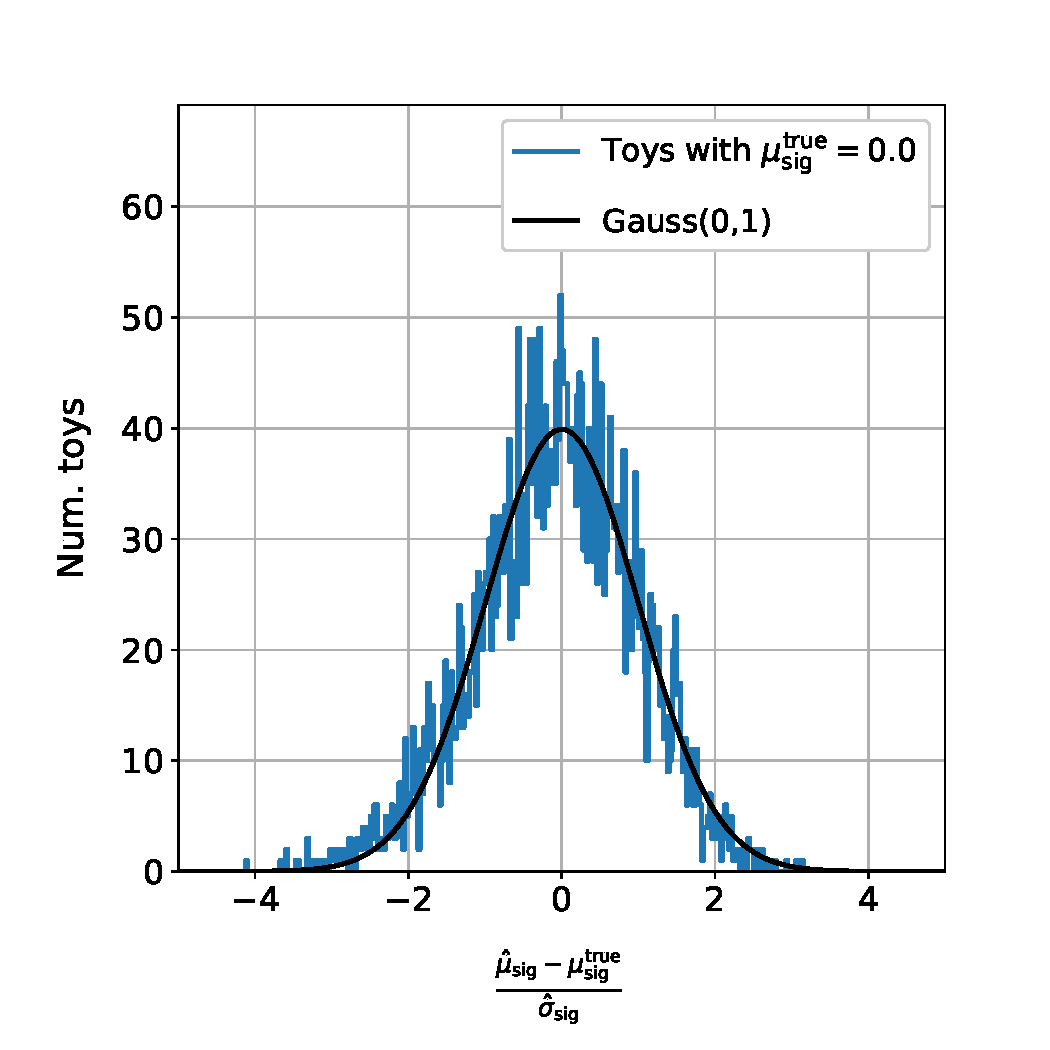
\includegraphics[page=1, width=0.49\textwidth]{Pulls.pdf}
\includegraphics[page=2, width=0.49\textwidth]{Pulls.pdf}
\caption{Distribution of pulls in 4000 toy datasets generated under the model 1 hypothesis with (left) $\mu_\text{sig}^\text{true}=0$ and (right) $\mu_\text{sig}^\text{true}=3$. Standard normal distributions are overlayed for comparison. Good agreement demonstrates a fit procedure with small bias and good coverage.}
\label{F. Pulls}
\end{figure}





\subsection{A note on bias and coverage in the real-world}
\label{S. CLsInAction::BiasCoverage2}

Section~\ref{S. CLsInAction::BiasCoverage} used toy datasets to demonstrate that the fit procedure provided unbiased estimates of the PoI with appropriate uncertainty coverage. This check should always be performed. However, it does not prove that the fit model itself is appropriate in the real-world. For this reason, we should always \textbf{bootstrap} the real-world dataset.

This means that we create psuedo-datasets by varying each datapoint within it's uncertainty\footnote{For an unbinned dataset, we can achieve the desired result by multiplying each datapoint by a Poisson weight with a mean of $1$.} (assuming e.g. Poisson or Gaussian probability densities as appropriate). In this case, we set $\mu_\text{ref}$ equal to the nominal measurement $\mu_\text{sig}^\text{obs}$ around which the fluctuations are applied. Significant deviations of the pull distribution from standard normal indicate that the fit model is not appropriate for the measured dataset. This complements other metrics of compatibility such as goodness-of-fit and NP pull tests.

In summary, the toy tests of Section~\ref{S. CLsInAction::BiasCoverage} should be performed to validate the statistical procedure. The bootstrapping approach of this section should be performed to validate the statistical model.





\subsection{Expected distribution of the test statistic}
\label{S. CLsInAction::TestStatDist}

Generating toy distributions was previously stated to be an effective method for deriving the expected distribution of the PoI pulls accounting for statistical variance. It is also an effective method for deriving the expected distribution of all other quantities. When we generate toys, we are introducing artificial statistical variations according to their expected probability densities, and can thus measure the spread induced on any measurable quantity.

For both the $CL_s$ and $CL_{s+b}$ methods, Figure~\ref{F. CL from test-stat} (left) demonstrated that we must know the expected distribution of the test statistic, $q$, for each possible value of $c_\text{model}=\mu_\text{sig}$. We derive this by generating toy datasets around the model expectation for each scan point in $\mu_\text{sig}$. Two such distributions are shown in Figure~\ref{F. q dist} using the \texttt{model 1} hypothesis under the $b$ hypothesis (left) and a typical scan point (right). When a value $q_\text{obs}$ is measured in a dataset, these distributions allow us to derive $CL_{b}$, $CL_{s+b}$ and thus $CL_s$ for each scan point in $\mu_\text{sig}$.


\begin{figure}[t!]
\centering
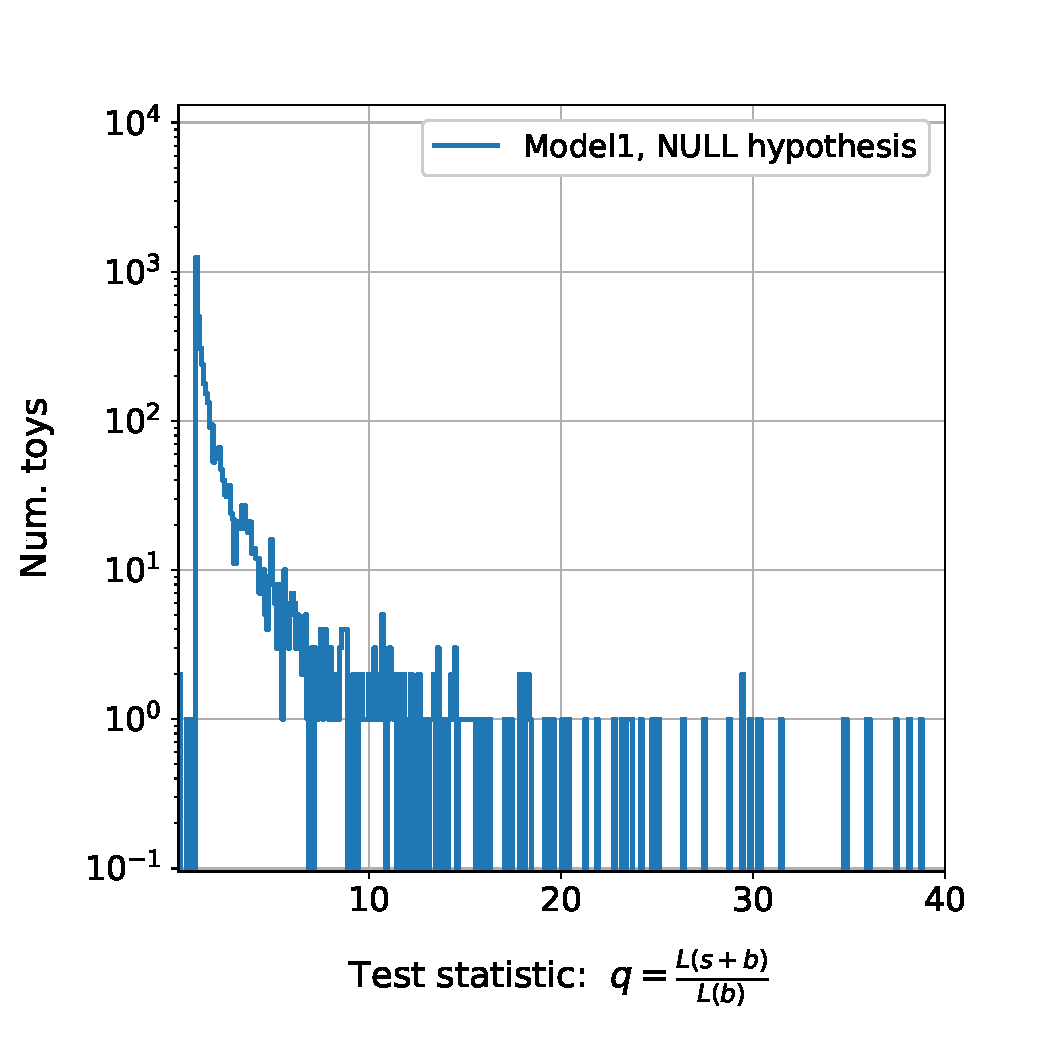
\includegraphics[page=1, width=0.49\textwidth]{TestStatisticToys.pdf}
\includegraphics[page=7, width=0.49\textwidth]{TestStatisticToys.pdf}
\caption{Expected distribution of the test statistic, $q$, evaluated using 4000 toy datasets generated at two different values of $\mu_\text{sig}^\text{true}$.}
\label{F. q dist}
\end{figure}





\subsection{Confidence levels}
\label{S. CLsInAction::ConfidenceLevels}

We are now equipped to evaluate confidence limits. The $CL_{s+b}$ and $CL_s$ profiles are evaluated in all toys. Two examples are shown in Figure~\ref{F. CL curve}. \texttt{Model 1} is used with two different values of $\mu_\text{sig}^\text{true}$. When $\mu_\text{sig}^\text{true}$ is sufficiently large, the $CL_s$ and $CL_{s+b}$ methods provide similar results. This is because all toy datasets are able to exclude the null hypothesis ($b$ only), therefore $\mathcal{L}_b \ll \mathcal{L}_{s+b}$, therefore $q_\text{obs}$ is usually large, therefore $CL_b\approx1~\forall~\mu_\text{sig}$. However, when $\mu_\text{sig}^\text{true}$ is zero, we find $CL_s \geq CL_{s+b}$. In this regime, $CL_s$ limits will be more conservative than the frequentist case.

Based on the shape of the $CL$ profiles in Figure~\ref{F. Coverage}, we can see our measurement will be presented as an upper limit on $\mu_\text{sig}$ if we define limits by excluding the region where $CL\leq95~\%$. We now test the coverage of the two methods. We use the following definition:

 \begin{table}[h!]
 \begin{tabular}{lc}
\multirow{2}{*}{\textbf{\emph{Expected coverage}}} \hspace{0.5cm}  & ``the fraction of toy datasets in which $\mu_\text{sig}^\text{true}$ was excluded with \\
& 95~\% confidence, i.e. for which $CL\left(\mu_\text{sig}=\mu_\text{sig}^\text{true}\right)<0.05$''
\end{tabular}
\end{table}

Using \texttt{model 1}, Figure~\ref{F. Coverage} shows the expected coverage of the $CL_s$ and $CL_{s+b}$ as a function of $\mu_\text{sig}^\text{true}$. Since $CL_{s+b}$ is truly frequentist, we confirm that the expected coverage is always 95~\% by definition. We see that $CL_s$ is conservative for small expected signals and ``overcovers''\footnote{It is not really ``overcovering'' if this is the intended behaviour!} compared with $CL_{s+b}$. As the expected signal increases and unambiguously excludes the null hypothesis, the coverage of $CL_s$ converges towards that of $CL_{s+b}$.

\begin{figure}[!]
\centering
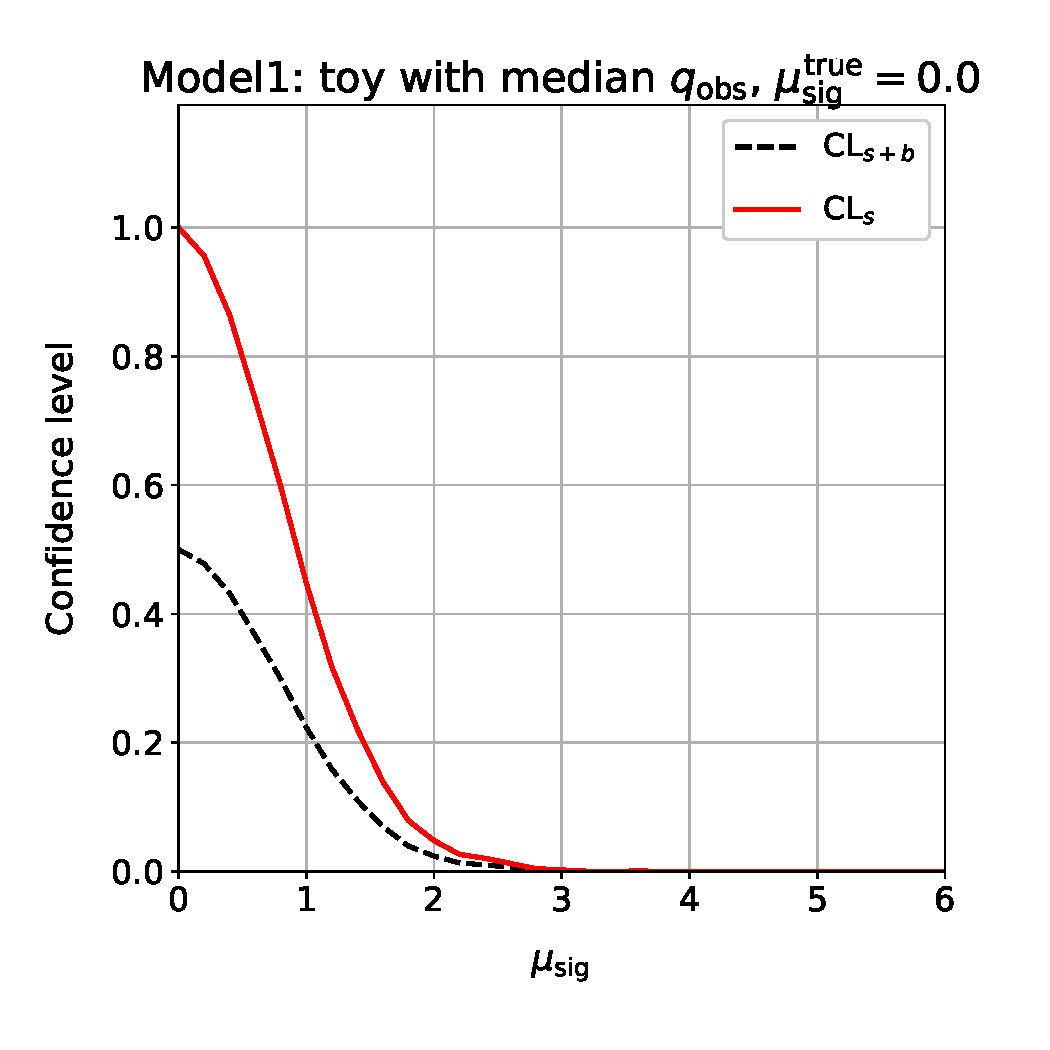
\includegraphics[page=1, width=0.49\textwidth]{CL_and_coverage.pdf}
\includegraphics[page=14, width=0.49\textwidth]{CL_and_coverage.pdf}
\caption{$CL_{s+b}$ and $CL_s$ curves evaluated using individual toys generated under two different $\mu_\text{sig}^\text{true}$ hypotheses using \texttt{model 1}. The toy with median $q_\text{obs}$ is shown.}
\label{F. CL curve}
\vspace{1cm}
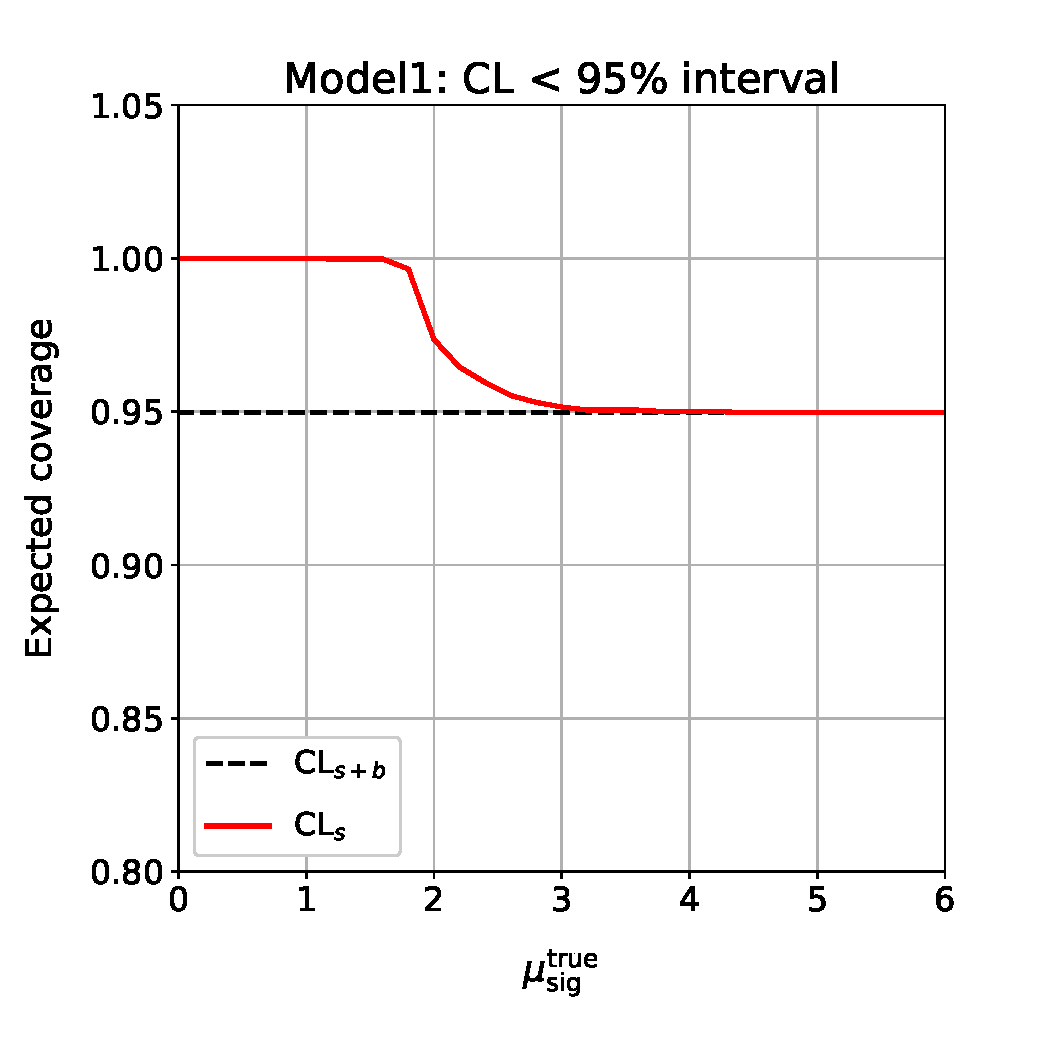
\includegraphics[page=1, width=0.63\textwidth]{Coverage.pdf}
\caption{Coverage of the $CL_{s+b}$ and $CL_s$ methods as a function of $\mu_\text{sig}^\text{true}$ using \texttt{model 1}.}
\label{F. Coverage}
\end{figure}







%\subsection{Summary}
%\label{S. CLsInAction::Summary}
%
%
%- toys --> check stat procedure is unbiased
%- toys --> expected distributions of q
%- toys --> expected coverage (optional)
%- data --> bootstrap to validate fit model
%- data --> 
%

